As a starting point, for our quest for a fast kNN search, our advisors gave us two papers by Garcia\citep{Garcia2008, Garcia2010}. The topic of these papers are to use a brute force method to solve the kNN problem. Expanding it into a All-kNN solution is then an easy task. These two papers is therefor a perfect start and introduces two new research questions.  

\begin{myrq}
Can high performance be achieved by a parallel brute force kNN algorithm on large point clouds.
\label{rq:brute_force_performance}
\end{myrq}

\begin{myrq}
Can a parallel brute force kNN algorithm be fast enough to solve the Q-kNN or All-kNN problem within reasonable time?
\label{rq:brute_force_Q-kNN}
\end{myrq}


% \subsection{Garcia's effort} % (fold)
\subsection{Garcia's path} % (fold)
\label{sub:garcia_s_effort}
 
Garcia's effort is based around a more mathematical version of our problem. A mathematician like to generalize a problem and make it a more uniform and accessible to other applications. For example, a mathematician does not make laws for only a 3-d space, but makes a more generalized version in the n-d space. In this case is is by widening the dimensions and not restricting the amounts of neighbors. In short, his problem is to find any number of closest neighbors in a space with any number of dimensions.  

His solution is based around a brute force method. In terms of parallel speedup this would be the best alternative to parallelize the kNN search, because the task can easily be divided into individual subtasks. The brute force, or exhaustive search, algorithm basically consists of three steps:

\begin{enumerate}
       \item Compute all distances between $q$ and all $m$ reference points in $S$.
       \item Sort the distances.
       \item Pick the $k$ shortest distances.
\end{enumerate}   


If this algorithm is to be used on $n$ query points the time complexity get an extinguishing, \BigO{nmd}. That sad, the parallelizable nature of the brute force method makes the speedup potentially high. Even though the speedup is great, and the parallelization is trivial, it does not imply that this is the best approach. Speedup is only a ratio between the parallel and serial speed, so if the algorithm itself is bad the parallel counterpart will also be affected. The brute force approach is steal an interesting candidate for our quest for a fast kNN search.


\subsection{Back on the right track} % (fold)
\label{sub:back_on_the_right_rrack}


Garcia's mathematical approach to the kNN problem is good and generic solution, but we need to take it towards a more specific path. Our problem, in regard to Garcia, is a more engineering-oriented problem. As engineers uses mathematical laws in a more specialized manner, we need to constrain Garcia's problem to fit our specifications. This include a 3-d space with a restricted number of $k$, as described in Section~\ref{a_short_introduction_to_kNN_search_problem}.


%TODO: Finne en bedre overskrift
% \subsubsection{The implementation} % (fold)
% \label{ssub:the_implementation}

First of all, Garcia's implementation only supports problem sizes up to $65535$, as our point clouds tends to be mush bigger, an expansion is therefore necessary. The limitation of $65535$ is exactly the number of theoretical blocks a kernel is allowed to spawn. An expatiation is therefore only a implementation issue, and is solved by a general partitioning algorithm. In short, the algorithm splits a list into a number of partitions. In this case, it is to partition the problem amongst different blocks, as visualized in Algorithm~\ref{alg:general_aspects_dividing}. The hole reimplementation of Garcia's algorithm can be found in Appendix~\ref{sec:brute_force_garcia}.

\begin{algorithm}[ht]
\caption{General work distribution in CUDA}
\label{alg:general_aspects_dividing}
\begin{algorithmic}
\State Let $L$ be any dividable work quantity of size $l$.
    \Function{CUDA-Kernel}{$L$}
    \State $b \gets blockIdx.x$ \Comment{Current block id.}
    \State $d \gets gridDim.x$ \Comment{Numbers of theoretical blocks in current grid.}
    \While{$b<l$}
    \State \Call{do-work}{$L(b)$}
    \State $b \gets b + d$
    \EndWhile
    \EndFunction
\end{algorithmic}
\end{algorithm}


A lot of improvements can be done with Garcia's algorithm, especially if we take advantage of our specialized case. For instance, with the dimension locked to three, the euclidean distance can be calculated in a mush easier fashion. Garcia, who has to take into account any number of dimensions, uses to vectors and cuBlas to calculate the distance. This makes a lot of extra complexity and data bandwidth, that can be ignored on our case.


An other, and the most time reducing improvement, has to to with the sorting step. On a problem instance with a small dimension, the most time consuming operation in Garcia's algorithm is the sorting operation. For instance, a search with $8$ dimensions, the sort occupies $62\%$ of the time. 

\subsubsection{Bitonic sort} % (fold)
\label{ssub:bitonic_sort}


The best sorting algorithm today has a time complexity of \BigO{mlog(m)}, which is a high price to pay for getting the smallest values in a list.  One could, as Garcia does, use a sorting algorithm that sorts the list in a linear fashion, where the smallest elements are sorted first. However, this property often gives the soring algorithm a bad time complexity. For instance, Garcia's insertion sort\cite{Cormen:2001} has a time complexity of \BigO{m^2}, and if it was used in our problem the time complexity of finding the $k$ smallest points would be \BigO{mk}. Asymptotically his would give a better timing results in cases where $k$ was smaller then $log(m)$. To get a better understanding of these numbers lets look at an example. If we analyze a case with a $k$ of around $100$. For the insertion sort to get any asymptoticly advantage over the best sorting algorithm, the problem size has to be bigger then $2^{100}$, which is a overwhelming $1.3e30$. We therefore think insertion sort is not the way to go.

Graham Nolan discusses the possibility of improving Garcia's algorithm by using bitonic sort, and he stats that it gave an significant impact\citep{Nolan}. Bitonic sort is a known \BigO{mlog(m)} algorithm, and is based around a soring network. The network is a series of interleaving bitonic sequences. A sequence is bitonic if it monotonically increases an then monotonically decreases\cite{Cormen:2001}. An iterative version of the bitonic sort is described in Algorithm~\ref{alg:bitonic_sort}.

\begin{algorithm}[ht]
\caption{Iterative Bitonic sort}
\label{alg:bitonic_sort}
\begin{algorithmic}
    \Require{A list $L$ with length $m$.}
    \Ensure{A sorted list, $L$}
    \State $P \gets \{2^i|i \in \mathcal{R}^+ \}$
    \Function{Bitonic-Sort}{$L$}
        \ForAll{$\{p \in P| p \in [2,m] \}$}
            \ForAll{ $\{k \in P| k \in [p,0]$}
                \ForAll{$i \in [0,m)$}
                \State $pos \gets k \veebar p$ \Comment{$\veebar$ is the bitwise $xor$ operator}
                \If{$pos < i$}
                    \If{$\lnot(i \& p)$} \Comment{$\&$ is the bitwise $and$ operator}
                        \State \Call{compare}{$L(i),L(pos)$}
                    \EndIf
                    \If{$(i \& p)$}
                        \State \Call{compare}{$L(pos),L(i)$}
                    \EndIf
                \EndIf
                \EndFor
            \EndFor
        \EndFor
    \EndFunction
    \Statex
    \Function{Compare}{$a,b$}
    \If{$a>b$}
    \State \Call{swap}{$a,b$}
    \EndIf
    \EndFunction
\end{algorithmic}
\end{algorithm}

% subsubsection bitonic_sort (end)

\subsubsection{Min-reduce} % (fold)
\label{ssub:min_reduce}

Sorting the distances, with a \BigO{mlog(m)} operations, steal looks like a high price to pay to get the smallest values. Especially if $k$ is reasonably small. Why do we need to sort the list in the first place? Sorting is a very naive way to go. The problem it solves is also extremely general compared to our specific goal, which is to get the smallest $k$ values. An algorithm that is more suitable, and also highly parallelizable, is a reduce operation. A $\otimes$-reduction of an array $d[1 \dots m]$, where $\otimes$ as any associative operator, is the value

     $$ y = d[1] \otimes d[2] \dots \otimes d[m].$$\cite{Cormen:2001}

In serial this is a typical linear algorithm with time complexity \BigO{m}, as shown in Algorithm~\ref{alg:serial_reduce}. 

\begin{algorithm}[ht]
\caption{Serial $\otimes$-reduction}
\label{alg:serial_reduce}
\begin{algorithmic}
    \State Let $\otimes$ be any associative operator.
    \Function{Reduce}{$d, \otimes$}
        \State $y \gets d[0]$
        \For{$i \gets 1,\, m$}
            \State $y \gets y \otimes d[i]$
        \EndFor
    \EndFunction
\end{algorithmic}
\end{algorithm}

Since the operator $\otimes$ is associative, there is no difference in which way the values are calculated or if it's done on parallel. A tree based approach, like Figure~\ref{fig:paralell_reduce_operation}, could be used. It is a good parallelization strategy, where every possible independent subtask is parallelized. Here each tree level do the associative operations in parallel, the results are combined as the tree level progresses, until only one element remains. The parallel equivalent to Algorithm~\ref{alg:serial_reduce} is therefore done in \BigO{log(n)} time. 

% TODO: finne en tittle
\begin{figure}[ht!]
\centering
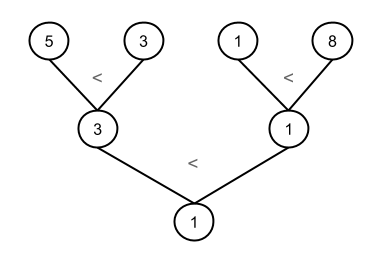
\includegraphics[width=50mm]{../gfx/min_reduce.png}

\caption{A visualization of the parallel min-reduce operation.}
\label{fig:paralell_reduce_operation}
\end{figure}

To solve our problem the associative operation has to be the minimal operator. A min-reduce algorithm is easy to implementation in CUDA, but it is hard to get fast. Some implementation techniques, like unrolling, sequential addressing and warp unrolling, described in Section~\ref{sec:cuda_optimizations}, is therefore necessary.   
% subsubsection min_reduce (end)

\subsubsection{Results} % (fold)
\label{ssub:comparison}

% subsubsection comparison (end)
Now that we have three different implementations of the kNN brute force method, lets take look at how they compete. Figure~\ref{fig:brute_force} shows the timing results with $k$ equals $10$. Garcia's algorithm lose mush time, because of the more general problem it solves. The generality also impacts the number of supported reference points, as the shorted graph implies. Graham Nolan's idea to improve the sorting algorithm gave a huge impact. It is almost five times faster then Garcia's implementation, shown in Table~\ref{tab:tabulated_results_from_brute_force}. Bitonic sort has a soring network that is suited for lengths that is a power of two, which give some pits in the graph. Partitioning of the list amongst the CUDA blocks also moved the pits a bit around.  


\begin{figure}[ht!]
\centering
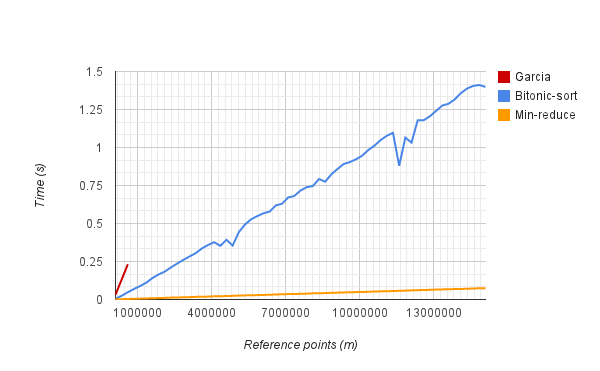
\includegraphics[width=100mm]{../gfx/brute_force.png}

\caption{Three different kNN brute force implementations. The timing results is based on a $k$ equal to $10$.}
\label{fig:brute_force}
\end{figure}




\begin{table}[ht]
\centering
    \begin{tabular}{ | l | l |l |l|}
    \hline
    \textbf{Reference points (m)} &\textbf{Garcia} & \textbf{Bitonic sort} & \textbf{Min-reduce}\\ \hline
    \textbf{\numprint{6.0e5}} & $231.8ms$ & $48.1ms$& $3.3ms$\\ \hline
    \textbf{\numprint{1.1e7}} & -& $1077.2ms$ & $54.2 ms$ \\ \hline
    \end{tabular}
    \caption{Some tabulated results from Figure~\ref{fig:brute_force}.}
    \label{tab:tabulated_results_from_brute_force}
\end{table}


The big winner in this contest is the min-reduce version. It is $70$ times faster then Garcia and almost $15$ times faster then the bitonic version. Although min-reduce is the big winner at a low k, lets not imply that it always is going to be the best alternative before some analysis are made.

First of all, lets see whats happening asymptoticly when $k$ is increasing.  Performing $k$ min-reduce operations takes \BigO{klog(m)} time, because one min-reduce has a time complexity of \BigO{log(m)}. If we increase $k$ towards $m$, the time complexity will go towards \BigO{mlog(m)}. This is the same time complexity as our bitonic sort. The asymptotic growth of the min-reduce variant will not be any different then the bitonic sort variant, even though $k$ equals $m$. 


The min-reduce naturally have more constant time penalties than the bitonic version. However, if $k$ is reasonably small, the min-reduce method is highly superior.   
% subsubsection the_implementation (end)



% subsection back_on_the_right_rrack (end)

 % subsection garcia_s_effort (end) 
